\documentclass{article}

\usepackage{minitoc}
\usepackage{tabularx}
\usepackage{booktabs}
\usepackage{graphicx}
\usepackage{hyperref}
\usepackage{xcolor}
\usepackage{blkarray}
\usepackage{amsthm, amssymb, amsmath}
\usepackage{caption}
\usepackage{subcaption}
\usepackage{multirow}
\usepackage[ruled,vlined]{algorithm2e}

\usepackage{natbib}
\bibliographystyle{abbrvnat}

\theoremstyle{definition}
\newtheorem{definition}{Definition}[section]
\newtheorem{theorem}{Theorem}[section]
\newtheorem{lemma}[theorem]{Lemma}
\newtheorem{conjecture}[theorem]{Conjecture}

\usepackage[margin=2.5cm, includefoot, footskip=30pt]{geometry}
\pagestyle{plain}
\setlength{\parindent}{0em}
\setlength{\parskip}{1em}

\renewcommand{\baselinestretch}{1}

\usepackage{standalone}

\newtheorem{proposition}{Proposition}

\title{$n-$bits reactive strategies}

\author{Nikoleta E. Glynatsi, Ethan Akin, Martin Nowak, Christian Hilbe}
\date{}

\begin{document}

\maketitle


\section{Introduction}

In this work we explore \textit{reactive strategies} in the infinitely repeated
prisoner's dilemma. The prisoner's dilemma is a two person symmetric game that
provides a simple model of cooperation. Each of the two players, \(p\) and
\(q\), simultaneously and independently decide to cooperate (\(C\)) or to defect
(\(D\)). A player who cooperates pays a cost \(c > 0\) to provide a benefit \(b
> c\) for the co-player. A cooperator either gets \(b\!-\!c\) (if the co-player
also cooperates) or \(-c\) (if the co-player defects). Respectively, a defector
either gets \(b\) (if the co-player cooperates) or 0 (if the co-player defects),
and so, the payoffs of player \(p\) take the form,

\begin{equation}\label{eq:donation_payoffs}
  \begin{blockarray}{ccc}
      & \text{cooperate} & \text{defect} \\
      \begin{block}{c(cc)}
          \text{cooperate} & b\!-\!c & -c \\
          \text{defect} & b & 0 \\
      \end{block}
  \end{blockarray}
\end{equation}

The transpose of (\ref{eq:donation_payoffs}) gives the payoffs of co-player
\(q\). We can also define each player's payoffs as vectors,

\begin{equation}\label{eq:vector_payoffs}
  \mathbf{S}_{p} = (b\!-\!c, -c, b, 0) \quad \textrm{and} \quad  \mathbf{S}_{q} = (b\!-\!c, b, -c, 0).
\end{equation}

\section{Model}

At each round $t$ of the repeated game, players \(p\) and \(q\) decide on an
action \(a^{p}_{t}, a^{q}_{t} \in \{C, D\}\) respectively (\textbf{Fig. 1a}). We
assume in the following, that the players' decisions only depend on the outcome
of the previous $n$ rounds. An {\it $n$-history for player $p$} is a string
$h^p=(a^p_{-1},\ldots,a^p_{-n})\!\in\!\{C,D\}^n$. An entry $a^p_{-k}$
corresponds to player $p$'s action $k$ rounds ago. Let $H^p$ denote the space of
all $n$-histories of player~$p$. Analogously, we define $H^q$ as the set of
$n$-histories $h^q$ of player~$q$. Sets $H^p$ and $H^q$ contain
$|H^p|=|H^q|=2^{n}$ elements each. A pair $h\!=\!(h^p,h^q)$ is called an {\it
$n$-history of the game}. We use $H=H^p\times H^q$ to denote the space of all
such histories. This set contains $|H|=2^{2n}$ elements. 

A {\it memory-$n$} strategy is a vector $\mathbf{p}=(p_h)_{h\in
H}\in[0,1]^{2n}$. Each entry $p_h$ corresponds to the player's cooperation
probability in the next round, depending on the outcome of the previous $n$
rounds.

Compared to this, a {\it $n-$ bit reactive strategy} is a vector
$\mathbf{\hat{p}}=(\hat{p}_h)_{h\in H^q}\in[0,1]^{2n}$. Each entry $p_h$
corresponds to the player's cooperation probability in the next round, depending
on the co-player's action(s) of the previous $n$ rounds. Thus, $n$-bit reactive
strategies only depends on the co-player's $n$-history (independent of the focal
player's own actions during the past $n$ rounds).

\begin{figure}[h!]
    \centering
    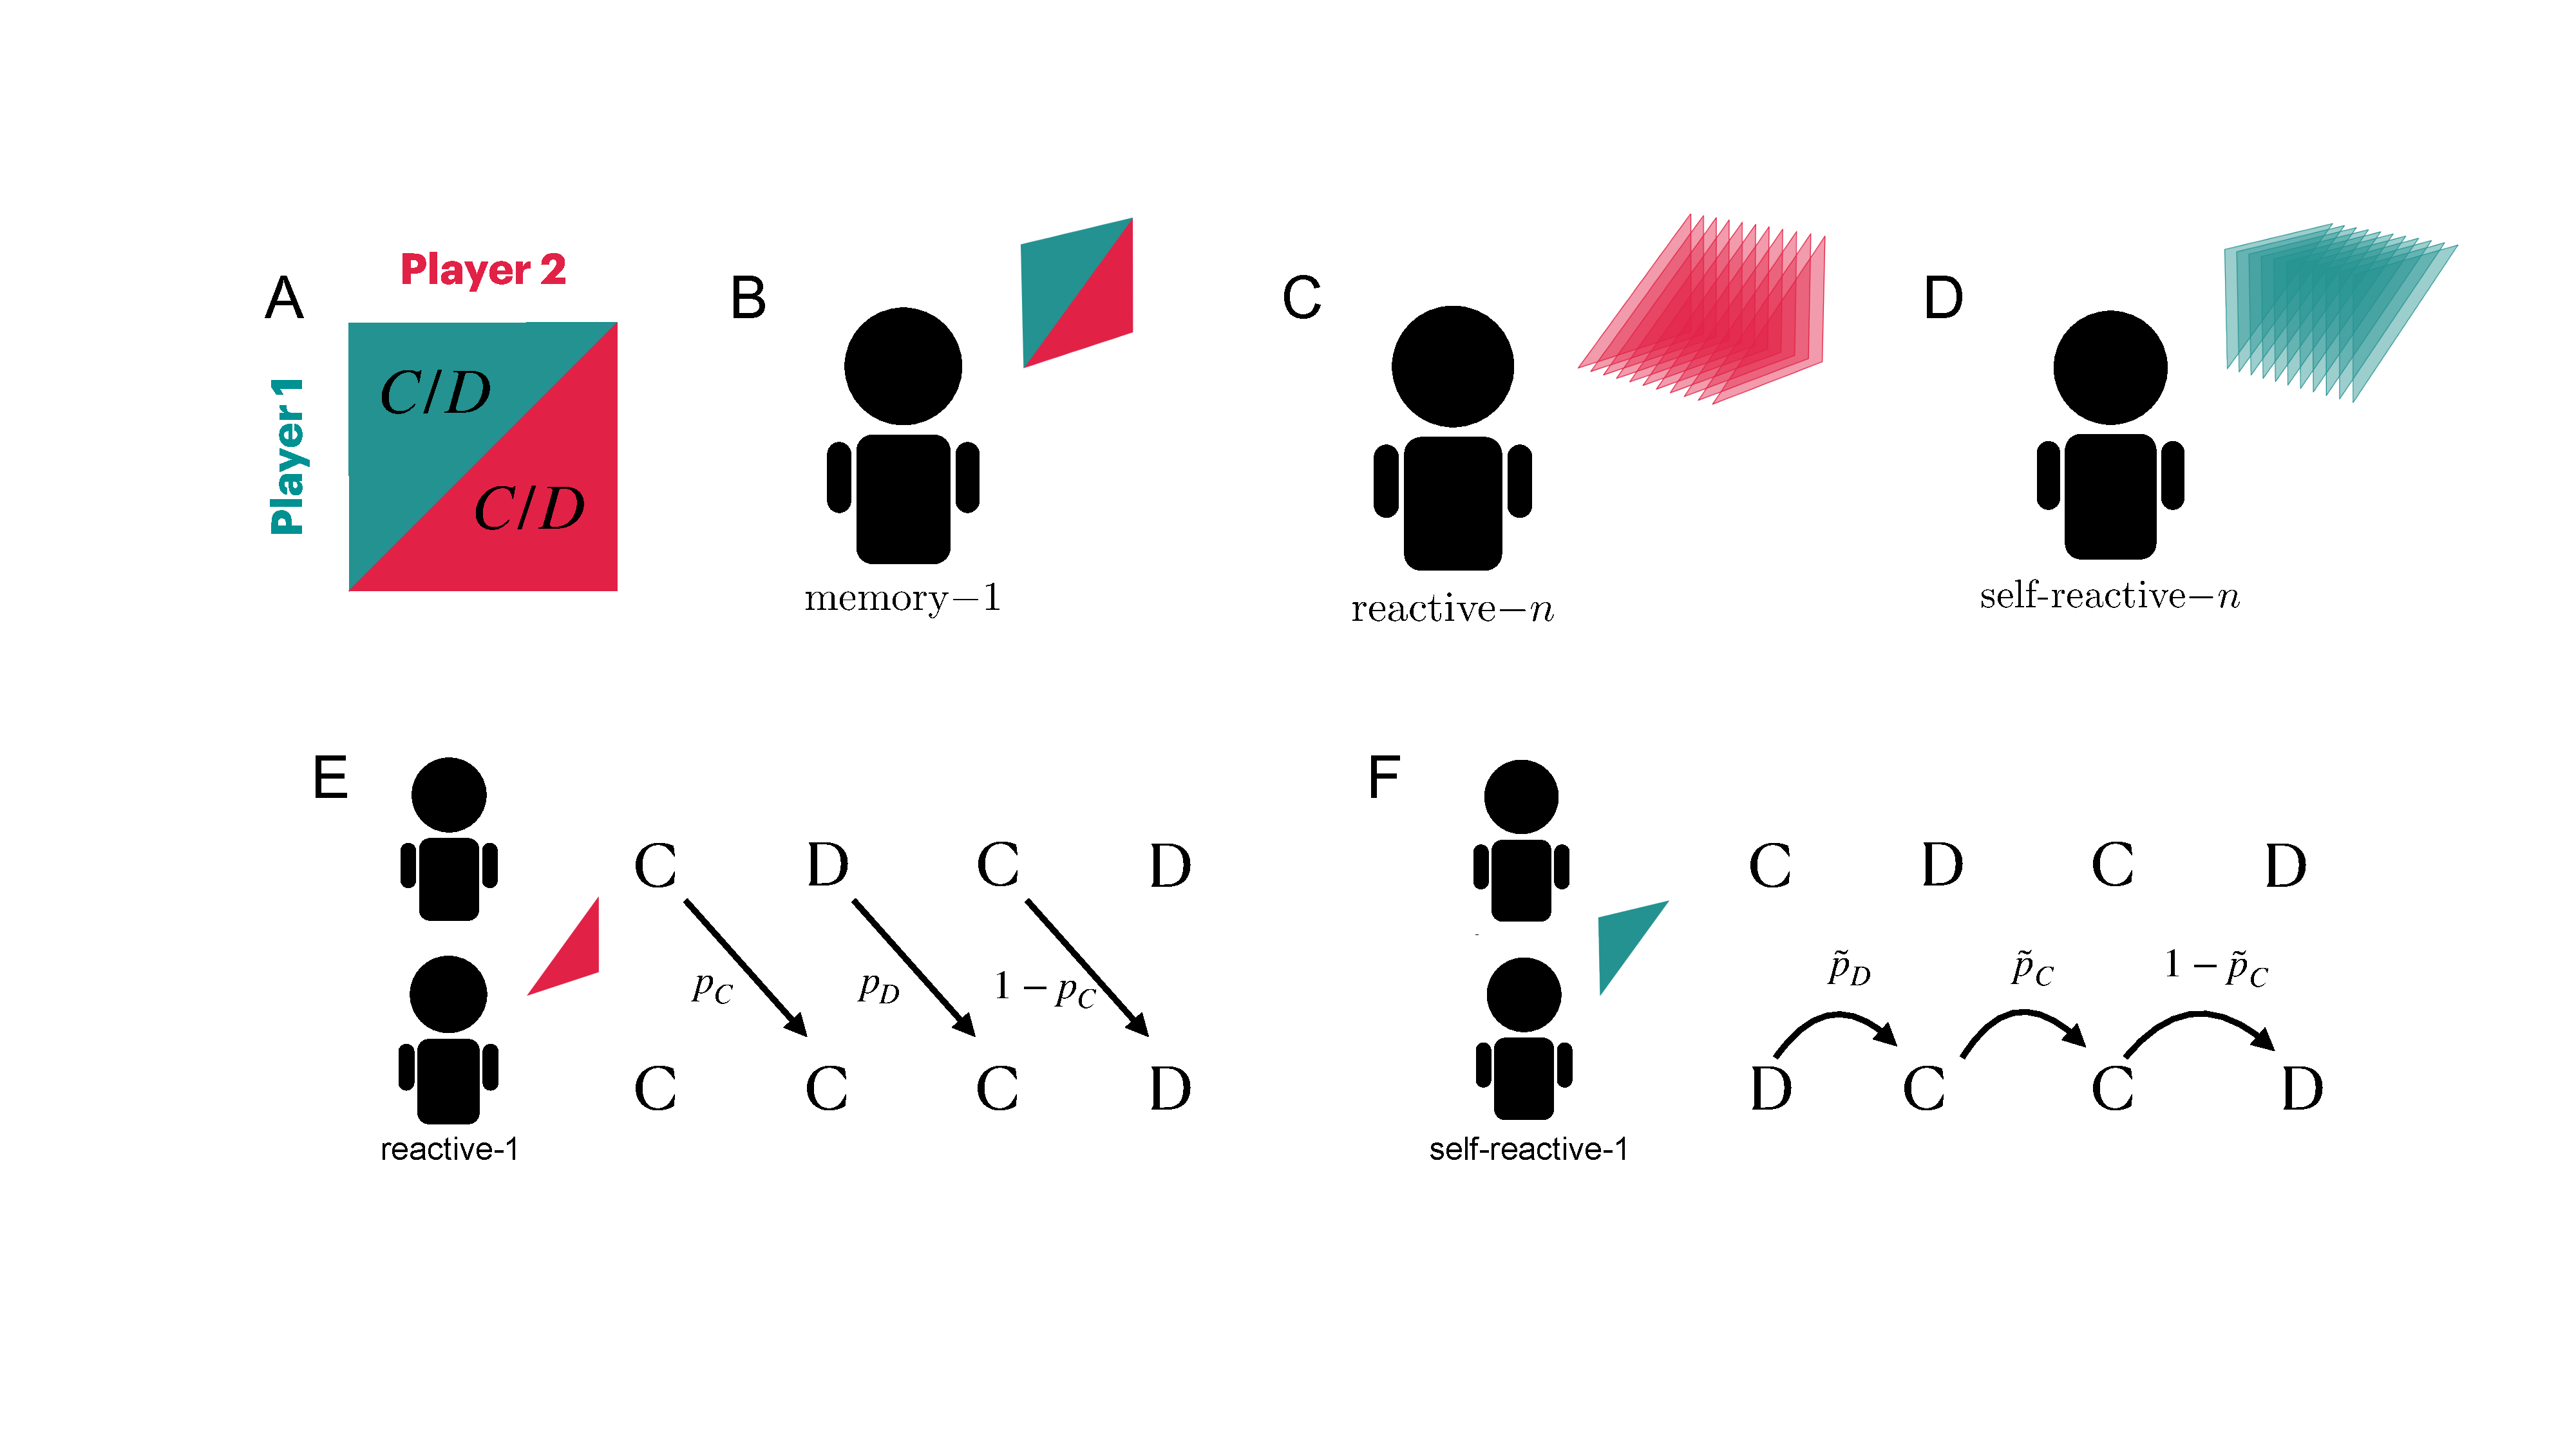
\includegraphics[width=\textwidth]{figures/conceptual_figure_model.pdf}
    \caption{\textbf{Model.} \textbf{a)} At each turn $t$ of the repeated game,
    players \(p\) and \(q\) decide on an action \(a^{p}_{t}, a^{q}_{t} \in \{C,
    D\}\) respectively. \textbf{b)} Memory$-1$ strategies are a set of very well
    studied strategies in the literature. They consider the actions of both
    players at time $t-1$ for their decisions at turn $t$. \textbf{c)} Here we
    will focus on reactive strategies. Strategies that consider only the
    co-players actions $H^q$. \textbf{e)} Consider the case of $n=1$. A $1-$bit
    reactive strategy is a vector $\mathbf{\hat{p}}=(\hat{p}_1, \hat{p}_2)$. A
    match between two $1-$bit reactive strategies is shown in the panel. The top
    player (player $\hat{p}$) cooperates with a probability $\hat{p}_1$ in the
    second round since the co-player cooperated in the first round, player
    $\hat{p}$ cooperates with a probability $\hat{p}_2$ in the second round
    since the co-player cooperated and defects with a probability $1 -
    \hat{p}_2$ given that the co-player defected again. \textbf{d)}We will also
    discuss the set of self reactive strategies}
\end{figure}

If the two players use memory-$n$ strategies $\mathbf{p}$ and $\mathbf{q}$, one
can represent the interaction as a Markov chain with a $2^{2n}\!\times\!2^{2n}$
transition matrix $M$. Let $\mathbf{v}=(v_h)_{h\in H}$ be an invariant
distribution of this Markov chain. 

{\bf Partner strategies.}  We say $h\!=\!(h^p,h^q)$ is the mutual cooperation
history if $h^p\!=\!h^q\!=\!(C,\ldots,C)$. A memory-$n$ strategy $\mathbf{p}$ is
called agreeable if it prescribes to cooperate with probability 1 after the
mutual cooperation history. The strategy $\mathbf{p}$ is called good if it is
agreeable and if expected payoffs satisfy
\begin{equation} \label{Eq:good}
    s_{\mathbf{q}} \geq b\!-\!c \qquad \Rightarrow \qquad s_{\mathbf{q}} = s_{\mathbf{p}} =  b\!-\!c,
\end{equation}

We wish to characterise all good memory-$n$ strategies of the repeated donation
game. To start with, in the following we begin with the simplest non-trivial
case.


\section{Results}

\subsection{Sufficiency of self reactive strategies}

To characterise all partner $n-$bit reactive strategies one would need to check
against all $n-$ memory one strategies. However, we show that when $p$ plays as
a $n-$bit reactive strategy then it suffices to check only against $n-$bit
self reactive strategies. This result is in line with the 
previous finding of Press and Dyson~\cite{press:PNAS:2012}.

More specifically, the result is that for any strategy memory-$n$, for player
\(q\), \(p\)'s score is exactly the same as if \(q\) had played a certain self
reactive memory-$n$ strategy.

\subsection{$2-$bit partner strategies}

For $n=2$, $\mathbf{\hat{p}}=(\hat{p}_1, \hat{p}_2, \hat{p}_3, \hat{p}_4)$ where
$\hat{p}_1$ is the probability of cooperating in round $t$ when the co-player
cooperates in the last 2 rounds. An agreeable $2-$bit strategy is of the
vector $\mathbf{\hat{p}}=(1, \hat{p}_2, \hat{p}_3, \hat{p}_4)$.

An agreeable $2-$bit reactive strategy is a partner strategy if the entries of
$\mathbf{\hat{p}}$ satisfy:

\begin{equation}\label{eq:two_bit_conditions}
  \displaystyle \hat{p}_{DD} < 1\!-\! \frac{c}{b}  ~~and~~ \displaystyle \frac{\hat{p}_{CD} + \hat{p}_{DC}}{2} < 1-\frac{c}{2b}.
\end{equation}

A special case of $2-$bit reactive strategies are {\it  $2-$bit counting
reactive strategies}. These are strategies that respond to the action of the
co-player but they do not differentiate between when the defection occur but if
a defection or two occurred. Let $r_i$ be the probability of cooperating given
that the co-player cooperated $i$ number of times in the last 2 turns.

Thus, $r_2 = \hat{p}_1, r_1 = \hat{p}_2 =  \hat{p}_3, r_0 = \hat{p}_4$ and
$\mathbf{\hat{p}}=(r_0, r_1, r_2)$.
Conditions~(\ref{eq:two_bit_conditions}) then become:

\begin{equation}\label{eq:counting_two_bit_conditions}
  \displaystyle r_2 < 1, \quad r_2 < 1-\frac{c}{2b} ~~and~~ r_0 < 1\!-\! \frac{c}{b}.
\end{equation}

\subsection{$3-$bit partner strategies}

For $n=3$, $\mathbf{\hat{p}}=(\hat{p}_1, \hat{p}_2, \hat{p}_3, \hat{p}_4,
\hat{p}_5, \hat{p}_6, \hat{p}_7, \hat{p}_8)$ where $\hat{p}_1$ is the
probability of cooperating in round $t$ when the co-player cooperates in the
last 23rounds. An agreeable $3-$bit strategy is of the vector
$\mathbf{\hat{p}}=(1, \hat{p}_2, \hat{p}_3, \hat{p}_4, \hat{p}_5, \hat{p}_6,
\hat{p}_7, \hat{p}_8)$.

An agreeable $3-$bit reactive strategy is a partner strategy if the entries of
$\mathbf{\hat{p}}$ satisfy:

\begin{align}\label{eq:three_bit_conditions}
  \hat{p}_{CCD} + \hat{p}_{CDC} + \hat{p}_{DCC} < 3\!-\! \frac{c}{3b}, \quad 
  \hat{p}_{CDD} + \hat{p}_{DDC} + \hat{p}_{DCD} < 3\!-\! \frac{2c}{b}, \quad \\
  \hat{p}_{CDC} + \hat{p}_{DDC} < 2\!-\! \frac{c}{b}, \quad \hat{p}_{CCD} + \hat{p}_{CDD} + \hat{p}_{DDC} +  \hat{p}_{DCD} < 4\!-\! \frac{2c}{b} ~~and~~ \hat{p}_{DDD} < 1\!-\! \frac{c}{b}.
\end{align}

A special case of $3-$bit reactive strategies are {\it  $3-$bit counting
reactive strategies}. These are strategies that respond to the action of the
co-player but they do not differentiate between when the defection occur but if
a defection or two or three occurred. Let $r_i$ be the probability of cooperating given
that the co-player cooperated $i$ number of times in the last 3 turns.

Thus, $r_3 = \hat{p}_1, r_2 = \hat{p}_2 =  \hat{p}_3, r_1 = \hat{p}_2 =  \hat{p}_3, r_0 = \hat{p}_4$ and
$\mathbf{\hat{p}}=(r_0, r_1, r_2, r_3)$.
Conditions~(\ref{eq:three_bit_conditions}) then become:

\begin{equation}\label{eq:counting_three_bit_conditions}
  \displaystyle r_3 < 1, \quad r_2 < 1-\frac{2c}{3b}, \quad r_1 < 1-\frac{c}{3b} ~~and~~ r_0 < 1\!-\! \frac{c}{b}.
\end{equation}


\subsection{$n-$bit counting partner strategies}

In the case of the counting reactive strategies we see a pattern to the
partner strategies conditions. We show that for an $n-$bit counting
reactive strategy to be a partner strategy then the strategy's entries
must satisfy the conditions $r_{i} < n - \frac{i \times c}{n b}$.

\subsection{Evolutionary Dynamics}

\section{Discussion}

~\\
\bibliography{bibliography.bib}

\end{document}